%%% 特別研究報告書サンプル
\documentclass[dvipdfmx]{ampbt}

%%% クラスオプション:
%%% chapter:   \chapterコマンドを使用可能にする(jsbook (report) を使う).
%%% その他 jsclasses に指定可能なオプションが指定できます(そのまま渡される).

%%% 題目 %%%%%%%%%%%%%%%%%%%%%%%%%%%%%%%%%%%%%%%%%%%%%%%%%%%%%%%%%%%%%%%%%%%%%%%%
\title{境界積分方程式方による音場の数値解析と}     % 題目1行目
      {移動する受音点におけるリアルタイム可聴化について}      % 題目2行目
      {}                                             % 題目3行目
%%% 指導教員 %%%%%%%%%%%%%%%%%%%%%%%%%%%%%%%%%%%%%%%%%%%%%%%%%%%%%%%%%%%%%%%%%%%%
\supervisors{吉川仁}{准教授}    % 指導教員1人目 {氏名}{職名}
            {}{}    % 指導教員2人目 {氏名}{職名}
            {}{}                % 指導教員3人目 {氏名}{職名}
%%% 入学年月 %%%%%%%%%%%%%%%%%%%%%%%%%%%%%%%%%%%%%%%%%%%%%%%%%%%%%%%%%%%%%%%%%%%%
\entrancedate{26}{4}            % {年(平成)}{月}
%%% 著者氏名 %%%%%%%%%%%%%%%%%%%%%%%%%%%%%%%%%%%%%%%%%%%%%%%%%%%%%%%%%%%%%%%%%%%%
\author{石床}{竜一}             % {姓}{名}
%%% 提出日 %%%%%%%%%%%%%%%%%%%%%%%%%%%%%%%%%%%%%%%%%%%%%%%%%%%%%%%%%%%%%%%%%%%%%%
\submissiondate{30}{1}{26}      % {年(平成)}{月}{日}
%%% 背表紙の出力枚数 %%%%%%%%%%%%%%%%%%%%%%%%%%%%%%%%%%%%%%%%%%%%%%%%%%%%%%%%%%%%
\def\numberofspines{1}
%%% 摘要 %%%%%%%%%%%%%%%%%%%%%%%%%%%%%%%%%%%%%%%%%%%%%%%%%%%%%%%%%%%%%%%%%%%%%%%%
\abstract{%
  本研究では,一つの音源に対し、このモデルを用いて効率
  的に卒業論文を作成するためのアルゴリズムを開発した.また,このアルゴリズムを用
  いて,実際に本報告を作成した.その結果,従来の自分で執筆する方法に比べて,65536
  倍効率的に卒業論文を作成することが可能であることが確認された.
}
%%% パッケージの読み込みや自分用のマクロの定義 %%%%%%%%%%%%%%%%%%%%%%%%%%%%%%%%%%
\usepackage{amsmath,amssymb}
\newcommand{\rme}{\mathrm{e}}

%%% 出力の制御 %%%%%%%%%%%%%%%%%%%%%%%%%%%%%%%%%%%%%%%%%%%%%%%%%%%%%%%%%%%%%%%%%%

%%% 本文を出力しない場合,次の行のコメントを外して下さい.
%% \outputbodyfalse

%%% 末尾に表紙,背表紙を出力しない場合,次の行のコメントを外して下さい.
%% \outputcoverfalse

%%% 末尾に提出用摘要を出力しない場合,次の行のコメントを外して下さい.
%% \outputabstractforsubmissionfalse

%%% ampbt.cls では表紙等の作成のために geometry パッケージを使用しているため,本文
%%% のレイアウトを変えるために \usepackage[...]{geometry} とすると Option clash が
%%% 発生します.何らかの理由で本文のレイアウトを変更したい場合は \geometry{...} を
%%% 使用して下さい.
%%% また,jsclasses を使用しているため,例えば 3cm を指定したい場合は 3truecm と書
%%% く必要があります.
%% \geometry{hmargin=3truecm,vmargin=2truecm}

\begin{document}
\ifoutputbody
%%% 中表紙,摘要,目次 %%%%%%%%%%%%%%%%%%%%%%%%%%%%%%%%%%%%%%%%%%%%%%%%%%%%%%%%%%
\makeinsidecover                % 中表紙
\makeabstract                   % 摘要
\maketoc                        % 目次
\setcounter{page}{1}            % 本文のページ番号を1から始める
%%% 本文 %%%%%%%%%%%%%%%%%%%%%%%%%%%%%%%%%%%%%%%%%%%%%%%%%%%%%%%%%%%%%%%%%%%%%%%%
\section{序論}
序論っす.%\cite{suuri2010}
\section{定式化}
\subsection{対象とする問題}
ある閉じた領域の外部$D$における、空間座標$x$, 時刻$t$を引数とするスカラー量$u(x,t)$についての
次の初期値境界値問題を考える.
\begin{align}
&\ddot{u}(x,t)-c^2 u_{,ii}(x,t)=0,\  x \in D,\ t>0 \\
&u(x,0)=0,\  x \in D \\
&\dot{u}(x,0)=0,\  x \in D \\
&u(x,0)=\hat{u}(x,t),\  x\  \mbox{on} \ S_D,\ t>0 \\
&\frac{\partial{u}}{\partial{n}} (x,t)=\hat{q}(x,t),\  x\  \mbox{on} \ S_N,\ t>0
\end{align}
ここに$(\ )_{,i}$は$\dfrac{\partial{}}{\partial{x_i}}$,
$(\dot{\ })$は$\dfrac{\partial{}}{\partial{t}}$,
$\dfrac{\partial{}}{\partial{n}}$は法線微分で$n_i \dfrac{\partial{}}{\partial{x_i}}$,
$n(x)$は境界上の点$x$における領域の外向き単位法線ベクトル,
$S$は領域$D$の境界で$S=S_D \cup S_N$,
$c$は波速である.

\subsection{解の境界積分方程式による表現}
次に, 初期値境界値問題の境界積分方程式法による解析について説明する.
初期値境界値問題の境界積分方程式による解は,三次元波動方程式の基本解
\begin{align}
&\Gamma(x,t) = \displaystyle \frac{\delta(t-\dfrac{|x|}{c})}{4\pi|x|}
\end{align}
を用いて
\begin{equation}
  \label{eq:境界積分方程式}
u(x,t) = \int\!\!\!\int \Gamma(x-y,t-s) \frac{\partial u}{\partial n}(y,s) - \int\!\!\!\int \frac{\partial \Gamma}{\partial n}(x-y,t-s) \hat{u}(y,s) ds dS
\end{equation}
と表すことができる.
ここに$\delta(x)$はDiracのデルタ関数,
$t$は時刻,
$x$は領域内部の点,
$y$は境界上の点である.

\subsection{境界積分方程式の近似}
本研究では,受音点の各時刻での数値を境界積分方程式法を用いてリアルタイムに計算するが,%リアルタイムっていうやつの言葉とか
決められた時間内に特定の処理を終えなければならない制約ができる.そのため式(\ref{eq:境界積分方程式})を近似することを考える.\par
まず式(\ref{eq:境界積分方程式})第一項は基本解を代入して
\begin{align}
\int\!\!\!\int \dfrac{\delta(t-s-\dfrac{|x-y|}{c})}{4\pi|x-y|} \frac{\partial u}{\partial n}(y,s)dsdS
&= \int\!\!\!\int \dfrac{\delta(t-s-\dfrac{|x-y|}{c})}{4\pi|x-y|} \hat{q}(y,s)dsdS\\
&= \int\!\!\! \dfrac{1}{4\pi|x-y|} \hat{q}(y,t-\dfrac{|x-y|}{c})dS
\end{align}
となる.ここで,境界の面積分についての用いる.境界面を三角形で分割し,その各面要素を$S_j$とし,その面積を$S_j$とする.
面積分における各面積要素の積分値のために要する値が全て重心での値と等しいとし,面積の大きさ$S_j$との積をとることで
その面積要素の積分値の近似とする.この近似を用いるとき重心の値を$( )^g$と表記すれば,
\begin{align}
\int\!\!\! \dfrac{1}{4\pi|x-y|} \hat{q}(y,t-\dfrac{|x-y|}{c})dS &= \sum_j \int\!\!\! \dfrac{1}{4\pi|x-y_j|} \hat{q}(y_j,t-\dfrac{|x-y_j|}{c})dS_j \nonumber \\
&=\sum_j \dfrac{1}{4\pi|x-y_j^g|} \hat{q}(y_j^g,t-\dfrac{|x-y_j^g|}{c})S_j
\end{align}
\par
次に,式(\ref{eq:境界積分方程式})第二項に基本解を代入したものを考える.
\begin{align}
\int\!\!\!\int \dfrac{\partial}{\partial n}\left( \dfrac{\delta(t-s-\dfrac{|x-y|}{c})}{4\pi|x-y|} \right) \hat{u}(y,s) ds dS
&= \int\!\!\!\int \dfrac{\partial}{\partial n}\left( \dfrac{\delta(t-s-\dfrac{|x-y|}{c})}{4\pi|x-y|} \right) \hat{u}(y,s) ds dS \nonumber \\
&= \int\!\!\!\int -n_i\dfrac{\partial}{\partial x_i}\left( \dfrac{\delta(t-s-\dfrac{|x-y|}{c})}{4\pi|x-y|} \right) \hat{u}(y,s) ds dS
\end{align}
式(\ref{eq:境界積分方程式})第一項と同様に三角形に境界面を分割すれば,
\begin{align}
\sum_j -n_i\dfrac{\partial}{\partial x_i}\int\!\!\!\int \left( \dfrac{\delta(t-s-\dfrac{|x-y_j|}{c})}{4\pi|x-y_j|} \right) \hat{u}(y_j,s) ds dS_j
\end{align}
ここで,時刻$t$を時間ステップ$n$と時間刻み幅$\Delta t$を用いて$t=n\Delta t$とする.ここで,境界量$\hat{u}(x,t)$の近似のため,
区分一定の空間内挿関$M^m(t)$を次のように定義する.
\begin{align}
  M^m(t) =
\begin{cases}
\; \dfrac{t}{\Delta t}-m+1,&\ (m-1)\Delta t \leq t \leq m\Delta t  \\
\; \dfrac{-t}{\Delta t}+m+1,&\ m\Delta t \leq t \leq (m+1)\Delta t  \\
\; 0, &\ \mbox{otherwise}
\end{cases}
\end{align}
これを用いると上式は
\begin{align}
\sum_j \sum_m -n_i\dfrac{\partial}{\partial x_i}\int\!\!\!\int_{(m-1)\Delta t }^{(m+1)\Delta t} \left( \dfrac{\delta(n\Delta t-s-\dfrac{|x-y_j|}{c})}{4\pi|x-y_j|} \right) \hat{u}(y_j,m\Delta t)M^m(s)dsdS_j
\end{align}
ここで$n\Delta t-s = \tau$とすれば,
\begin{align}
\sum_j \sum_m -n_i\dfrac{\partial}{\partial x_i}\int\!\!\!\int_{(n-m-1)\Delta t }^{(n-m+1)\Delta t} \left( \dfrac{\delta(\tau- \dfrac{|x-y_j|}{c})}{4\pi|x-y_j|} \right) \hat{u}(y_j,m\Delta t)M^m(n\Delta t - \tau)d\tau dS_j \nonumber \\
\label{eq:Ndounyuumae}
= \sum_j \sum_m -n_i\dfrac{\partial}{\partial x_i}\int\!\!\!\int_{(n-m-1)\Delta t }^{(n-m+1)\Delta t} \left( \dfrac{\delta(\tau- \dfrac{|x-y_j|}{c})}{4\pi|x-y_j|} \right) \hat{u}(y_j,m\Delta t)M^{n-m}(\tau)d\tau dS_j
\end{align}
となる.ここで,$N^m(t)$を次のように定義する.
\begin{align}
  N^m(t) =
\begin{cases}
\; -\dfrac{t}{\Delta t}+m,&\ 0 \leq t \leq m\Delta t  \\
\; 0, &\ \mbox{otherwise}
\end{cases}
\end{align}
$N^m(t)$を用いて式(\ref{eq:Ndounyuumae})を書き換えると,
\begin{align}
\label{eq:Ndounyuu}
&\sum_j \sum_m -n_i\dfrac{\partial}{\partial x_i}\int\!\!\!  \int_{0}^{(n-m+1)\Delta t} \left( \dfrac{\delta(\tau- \dfrac{|x-y_j|}{c})}{4\pi|x-y_j|} \right) \hat{u}(y_j,m\Delta t)N^{n-m+1}(\tau)d\tau dS_j \nonumber\\
&\hspace{2em} +2n_i\dfrac{\partial}{\partial x_i}\int\!\!\!  \int_{0}^{(n-m)\Delta t} \left( \dfrac{\delta(\tau- \dfrac{|x-y_j|}{c})}{4\pi|x-y_j|} \right) \hat{u}(y_j,m\Delta t)N^{n-m}(\tau)d\tau dS_j \nonumber \\
&\hspace{2em} -n_i\dfrac{\partial}{\partial x_i}\int\!\!\!  \int_{0}^{(n-m-1)\Delta t} \left( \dfrac{\delta(\tau- \dfrac{|x-y_j|}{c})}{4\pi|x-y_j|} \right) \hat{u}(y_j,m\Delta t)N^{n-m-1}(\tau)d\tau dS_j \nonumber\\
&= \sum_j \sum_m -n_i\dfrac{\partial}{\partial x_i}\int\!\!\! \dfrac{( (n-m+1)\Delta t - \dfrac{|x-y_j|}{c} )H((n-m+1)\Delta t - \dfrac{|x-y_j|}{c} )}{4\pi|x-y_j|\Delta t} \hat{u}(y_j,m\Delta t) dS_j \nonumber\\
&\hspace{2em} +2n_i\dfrac{\partial}{\partial x_i}\int\!\!\!  \dfrac{( (n-m)\Delta t- \dfrac{|x-y_j|)}{c} )H((n-m)\Delta t - \dfrac{|x-y_j|}{c} )}{4\pi|x-y_j|\Delta t}  \hat{u}(y_j,m\Delta t) dS_j \nonumber \\
&\hspace{2em} -n_i\dfrac{\partial}{\partial x_i}\int\!\!\!  \dfrac{( (n-m-1)\Delta t - \dfrac{|x-y_j|)}{c} )H((n-m-1)\Delta t - \dfrac{|x-y_j|}{c})}{4\pi|x-y_j|\Delta t}  \hat{u}(y_j,m\Delta t) dS_j
\end{align}
ここに,$H(x)$はHeavisideの階段関数である.式(\ref{eq:Ndounyuu})に対して,第一項に行ったように重心の値を代表値として近似を用いれば,
\begin{align}
\label{eq:ヘヴィサイド後}
&\sum_j \sum_m -n_i\dfrac{\partial}{\partial x_i} \left(\dfrac{( (n-m+1)\Delta t - \dfrac{|x-y^g_j|}{c} )H((n-m+1)\Delta t - \dfrac{|x-y^g_j|}{c} )}{4\pi|x-y^g_j|\Delta t} \hat{u}(y^g_j,m\Delta t) S_j \right) \nonumber\\
&\hspace{2em} +2n_i\dfrac{\partial}{\partial x_i}\left(\dfrac{( (n-m)\Delta t- \dfrac{|x-y^g_j|)}{c} )H((n-m)\Delta t - \dfrac{|x-y^g_j|}{c} )}{4\pi|x-y^g_j|\Delta t}  \hat{u}(y^g_j,m\Delta t) S_j \right) \nonumber \\
&\hspace{2em} -n_i\dfrac{\partial}{\partial x_i}\left(\dfrac{( (n-m-1)\Delta t - \dfrac{|x-y^g_j|)}{c} )H((n-m-1)\Delta t - \dfrac{|x-y^g_j|}{c})}{4\pi|x-y^g_j|\Delta t}  \hat{u}(y^g_j,m\Delta t) S_j \right) \nonumber \\
=&\sum_j \sum_m \dfrac{n_i(x_i-y^g_i)}{4\pi \Delta t |x-y^g_j|^3}  \hat{u}(y^g_j,m\Delta t)(T^+H(T^+)-2TH(T)+T^-H(T^-) ) S_j  \nonumber\\
\end{align}
となる.ただし$T^+ =(n-m+1)\Delta t,\ T =(n-m)\Delta t,\ T^- =(n-m-1)\Delta t$である.
mについての値を陽に表記すると式(\ref{eq:ヘヴィサイド後})は
\begin{align}
\begin{cases}
\; \displaystyle\sum_j \sum_m \dfrac{n_i(x_i-y^g_i)}{4\pi \Delta t |x-y^g_j|^3}  \hat{u}(y^g_j,m\Delta t)(n-m+1)\Delta t S_j, &\dfrac{r}{c} < (n-m+1)\Delta t < \dfrac{r}{c}+\Delta t \nonumber\\  \\
\; \displaystyle\sum_j \sum_m \dfrac{n_i(x_i-y^g_i)}{4\pi \Delta t |x-y^g_j|^3}  \hat{u}(y^g_j,m\Delta t)(m-n+1)\Delta t S_j, &\dfrac{r}{c}+\Delta t < (n-m+1)\Delta t < \dfrac{r}{c}+2\Delta t \nonumber\\  \\
\; 0, &\ \mbox{otherwise}
\end{cases}
\end{align}
となり,上記近似により式(\ref{eq:境界積分方程式})第二項の計算量を大幅に減らすことができる.\par
以上の結果をまとめると,式(\ref{eq:境界積分方程式})は


% \begin{equation}\label{eq:student}
%   x(t)=x_0 \rme^{-t/a}.
% \end{equation}
% ここで,$x_0$は初期時刻$t=0$での学生のやる気,$a>0$は学生の研究への意欲を表す.
% 図~\ref{fig:student}はこのモデルによる学生のやる気の時間変化を$x_0=1$, $a=1$として
% プロットしたものである.
% \begin{figure}[htbp]
%   \centering
%   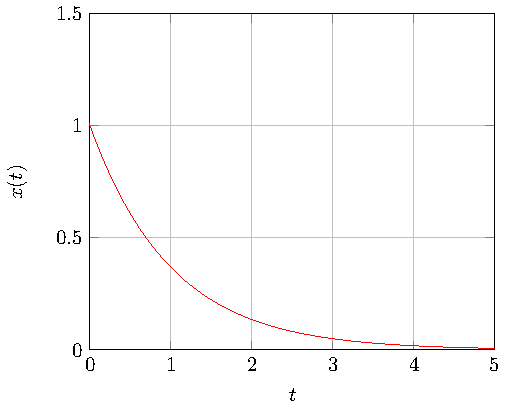
\includegraphics{ampbt_figure.pdf}
%   \caption{モデル\eqref{eq:student}による$x_0=1$, $a=1$のときの学生のやる気の時間
%     変化.}
%   \label{fig:student}
% \end{figure}
%
% モデル\eqref{eq:student}については,次のような問題点がある.
% \begin{itemize}
% \item 研究の進み具合や休憩によってやる気が復活する効果が考慮されていない.
% \item 締切が迫ってきたときのラストスパートが反映されていない.
% \end{itemize}




\subsection{卒業論文のモデル化}
…….

\section{効率的なアルゴリズムの開発}
本節では,前節までの結果を用いて,効率的に卒業論文を作成するためのアルゴリズムを開
発する.
…….

\section{結論}
本研究では,卒業論文を執筆する学生の数理モデルを構築した.

とりあえず境界積分方程式法を用いてがんばってけいさんしてみたけどクッソ遅かった。
的な状況が結論になりそうですね。

今後の課題としては,修士論文にもこのアルゴリズムを適用することが考えられる.

%%% 謝辞 %%%%%%%%%%%%%%%%%%%%%%%%%%%%%%%%%%%%%%%%%%%%%%%%%%%%%%%%%%%%%%%%%%%%%%%%
\acknowledgment
本研究に取り組むにあたって助言をいただいた吉川仁准教授に深く感謝
する.

%%% 参考文献 %%%%%%%%%%%%%%%%%%%%%%%%%%%%%%%%%%%%%%%%%%%%%%%%%%%%%%%%%%%%%%%%%%%%
\addcontentsline{toc}{section}{\refname} % 目次に参考文献を追加する.
                                         % chapter使用時は削除すること.
\begin{thebibliography}{10}
\bibitem{polya1945}
  G.~Polya, \textit{How to solve it: a new aspect of mathematical method},
  Princeton University Press, Princeton, 1945.
\bibitem{suuri2010}
  数理花子,数理モデルとその妥当性の検討,
  京都大学工学部情報学科数理工学コース特別研究報告,2010.
\end{thebibliography}
%%% BibTeX 等を用いる場合は,上の thebibliography 環境を消してここに該当コードを
%%% 挿入すること.
%% \bibliographystyle{...}
%% \bibliography{...}

%%% 付録 %%%%%%%%%%%%%%%%%%%%%%%%%%%%%%%%%%%%%%%%%%%%%%%%%%%%%%%%%%%%%%%%%%%%%%%%
%%% 付録は不要ならば削除してよい.
\appendix

\section{意味のない付録}
これは意味のない付録です.これは意味のない引用です\cite{polya1945}.

\begin{table}[htbp]
  \caption{これは意味のない表です.}
  \centering
  \begin{tabular}{c|cc}
      &  A  &  B \\
    \hline
    C &  70 & 80 \\
    D & 100 &  0
  \end{tabular}
\end{table}

%%% 本文ここまで %%%%%%%%%%%%%%%%%%%%%%%%%%%%%%%%%%%%%%%%%%%%%%%%%%%%%%%%%%%%%%%%
\fi
\ifoutputcover
\cleardoublepage
%%% 表紙,背表紙,提出用摘要 %%%%%%%%%%%%%%%%%%%%%%%%%%%%%%%%%%%%%%%%%%%%%%%%%%%%
\makecover                      % 表紙
\makespine[\numberofspines]     % 背表紙
\fi
\ifoutputabstractforsubmission
\makeabstractforsubmission      % 提出用摘要
\fi
\end{document}
